%!Tex root = Linguaggi.tex

\chapter{Introduzione}
Il problema principale dell'informatica consiste nel voler far eseguire ad una macchina algoritmi che manipolano dati.

\begin{figure}[H]
    \centering
    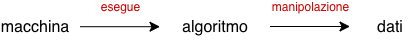
\includegraphics[width=0.6\textwidth]{images/linguaggi.png}
\end{figure}

Il primo meccanismo che viene associato alla storia dei computer è la \textbf{macchina di Babbage}, che può essere visto come il primo "computer" perchè nasce per eseguire calcoli matematici complessi in modo automatico.\\[0.2ex]
Sucessivamente, c'è un'evoluzione e il computer viene riconosciuto come macchina programmabile (dare delle istruzioni alla macchina per ottenere un determinato risultato).\\[0.2ex]
In questo contesto nasce \textbf{Enigma}, uno strumento per decodificare un codice mediante un algoritmo di forza bruta che tenta tutte le combinazioni.

La prima archiettura che darà origine all'archiettura dei computer moderni è l'\textcolor{colore}{\textbf{architettura di Von Neumann}}, un'achitettura hardware che comprende solo il linguaggio binario, un linguaggio costituito esclusivamente da stringhe di bit (o e 1) e che può essere utilizzato per codificare qualunque altro linguaggio, ma non è comprensibile dall'essere umano.\\[0.2ex]
Questo fa si che l'uomo per poter interagire e programmare macchine, necessita di un'evoluzione dei linguaggi, ha bisogno di costruire un linguaggio comprensibile in modo più immediato.

\section{Perchè studiare i PL?}
Le motivazioni sono diverse:
\begin{itemize}[label=$\triangleright$, itemsep=\smallskipamount]
    \item miglioarre la capacitò di esprimere idee in forma algoritmica
    \item scegliere appropriatamente un linguaggio
    \item migliorare la capacità di studiare o progettare nuovi linguaggi o costrutti
    \item comprendere meglio il significato dell'implementazione dei linguaggi di programmazione
\end{itemize}

\section{Cosa sono i PL?}
La nascita e l'evoluzione dei linguaggi di programmazione è, anche, dovuto, all'archiettura della macchina che bisogna programmare.

I computer moderni nascono dall'archiettura di Von Neumann.\\[0.2ex]
Questa è una tipologia di architettura hwardware con progrmma memorizzato, dove i dati e istruzioni condividono la stessa area di memoria.

\begin{figure}[H]
    \centering
    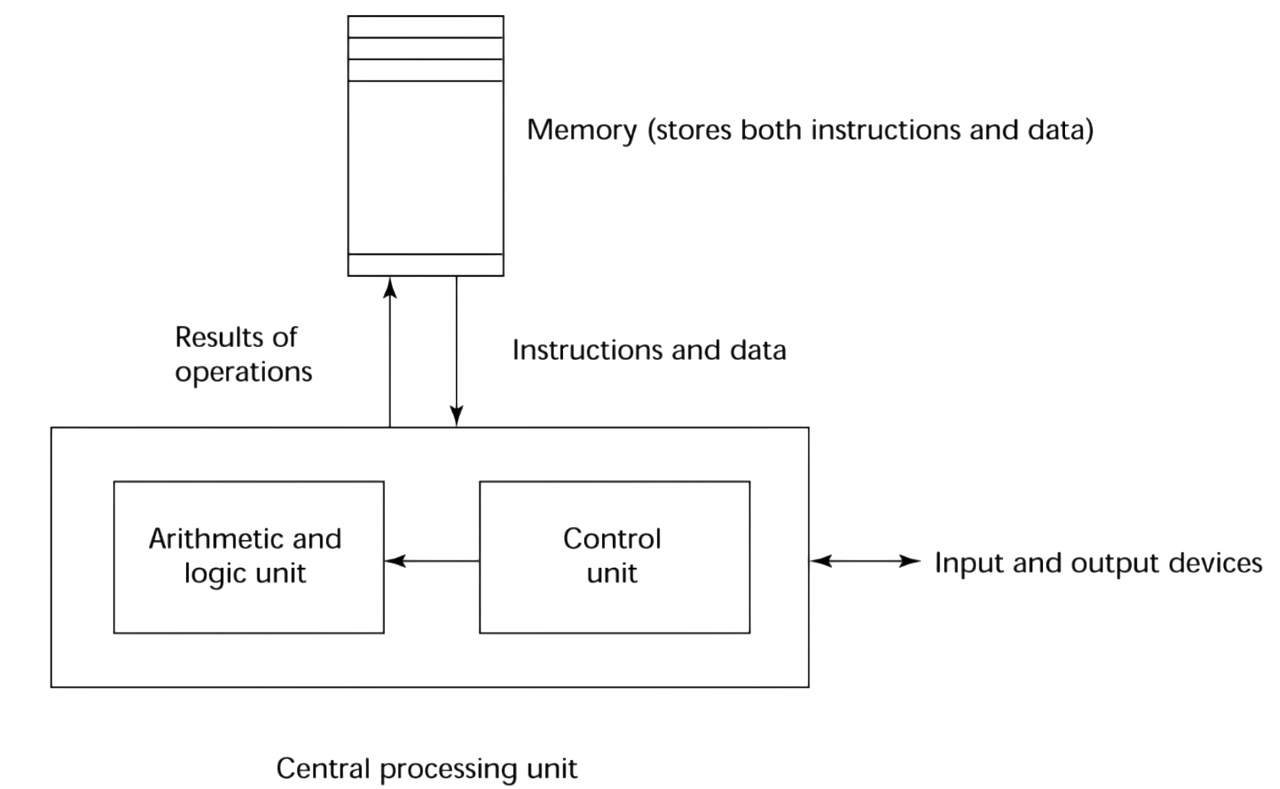
\includegraphics[width=0.6\textwidth]{images/architettura-von-neumann.png}
\end{figure}

\section{Cosa significa programmare?}
Il libguaggio di programmazione deve essere uno strumento che perette di descrivere algoritmi e rappresentare i dati.

\begin{figure}[H]
    \centering
    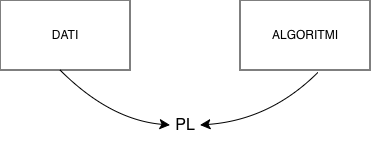
\includegraphics[width=0.5\textwidth]{images/linguaggio-programmazione.png}
\end{figure}

Il linguaggio binario è un linguaggio di programmazione in quanto permette di rappresentare algoritmi e dati , ma non è umanamente utilizzabile o interpretabile, in quanto potrebbe essere usata come dato o un dato interpretato come istruzione.\\[0.2ex]
Ciò significa, che un linguaggio di programmazione deve permettere di superare queste difficoltà, fornendo una chiara distinzione tra dato e istruzione.

\begin{mydef}{algoritmo}
    Un \textbf{algoritmo} è una sequenza infinta di passi di computazione, ovvero scompone un calcolo complesso in passi elementari.
\end{mydef}

Un algoritmo è un concetto astratto che trova forma concreta in un programma (sequenza finita di istruzioni).

\begin{mydef}{dati}
    I \textbf{dati} sono informazioni memorizzate concretamente in celle di memoria e astratte in elementi che il linguaggio può manipolare (variabili).
\end{mydef}

\begin{mydef}{programma}
    Un \textbf{programma} è la concretizzazione di un algoritmo che manipola dati.
\end{mydef}

\begin{mydef}{linguaggio di programmazione}
    Un \textbf{linguaggio di programmazione} è una notazione per scrivere un programma, ovvero serve a dare forma concreta agli algoritmi.
\end{mydef}

Il programma, quindi, costituisce la \textcolor{colore}{\textbf{sintassi}}.

Un programma è necessariamente un oggetto finito (sempre concreto), mentre il calcolo di una funzione richiede l'esecuzione di un insieme di passi primitivi, che, però possono essere infiniti.\\[0.2ex]
Ciò significa che un programma è una rappresentazione finita di un insieme, potenzialmente infinito, di passi primitivi di computazione.

\vario{Nota}{
    I linguaggi di programmazione devono dare specifica finita di oggetti potenzialmente infiniti.
}

\section{Contesti di sviluppo}
Il contesto in cui il linguaggio deve operare determina le funzionalità che deve gestire efficacemente:
\begin{itemize}[label=$\triangleright$, itemsep=\smallskipamount]
    \item \textbf{applicazioni scentifiche} (es. $\verb|Fortran|$)
    \item \textbf{applicazioni economiche} (es. $\verb|COBOL|$)
    \item \textbf{applicazioni artificiali} (es. $\verb|LISP|$)
    \item \textbf{programmazione di sistemmi} (es. $\verb|C|$)
    \item \textbf{web software} (es. $\verb|HTML|$ (markup), $\verb|PHP|$ (scripting), ecc.)
\end{itemize}

\section{Classificazione dei PL}
I linguaggi di programmazione si possono classificare in:
\begin{itemize}[label=$\diamond$, itemsep=\smallskipamount]
    \item \textcolor{colore}{\textbf{basso livello}}: linguaggi con caratteristiche specifiche dipendenti dall'architettura che si sta programmando (es. $\verb|linguaggio binario|$, $\verb|Assembly|$)
    \item \textcolor{colore}{\textbf{alto livello}}: linguaggi che permettono una programmazione strutturata in cui dati e istruzioni hanno rappresentazioni diverse
\end{itemize}

I linguaggi ad alto livello si possono classificare in base a:
\begin{itemize}[label=$\circ$, itemsep=\medskipamount]
    \item \textbf{paradigma di programmazione}
    \begin{itemize}[itemsep=\smallskipamount]
        \item linguaggi procedurali: codice diviso in subrutine che eseguono compiti semplici basati su salti condizionali (goto) [es. $\verb|COBOL|$]
        \item linguaggi strutturati (imperativi): procedurale senza goto (es. $\verb|C|$, $\verb|Pascal|$, $\verb|ADA|$, ec..)
        \item libguaggi orientati agli oggetti: classe elemento centrale della programmazione.
        Un linguaggio deve avere tre proprietà:
        \begin{itemize}[itemsep=\smallskipamount]
            \item incapsulamento
            \item eriditarietà
            \item polimorfismo
        \end{itemize}
        \item linguaggi dichiatirativi: basati su componenti della matematica
        \begin{itemize}[itemsep=\smallskipamount]
            \item logici: basati sulla logica proposizionale del primo ordine, in cui si effettuano calcoli tramite dimostrazione di datti (es. $\verb|PROLOG|$)
            \item matematici: basati sul concetto di applicazione di funzione (es. $\verb|LSIP|$, $\verb|ML|$)
        \end{itemize}
    \end{itemize}
    \item \textbf{termini gerazionali}
    \begin{itemize}[itemsep=\smallskipamount]
        \item I° generazione:
        \begin{center}
            $\downarrow$
        \end{center}
        \item II° generazione:
    \end{itemize}
\end{itemize}

\section{Implementazione di un PL}
Implementare un linguaggio significa eseguire un programma nel lingugaggio di programmazione in una macchina.\\[0.2ex]
Sicuramente, il modo in cui deve essere implementato è direttamente collegato all'architettura che deve programmare, ma anche al paradigma (metodologie) che il linguaggio di programmazione utilizza per costruire programmi.

\smallskip
Implementare un linguaggio significa realizzare la macchina (astratta) che interpresta il linguaggio.

\vario{Nota}{
    La macchina è astratta perchè, per rappresentare la macchina fisica (concreta), utilizza un linguaggio che è più astratto del linguaggio binario.
}

\begin{mydef}{macchina astratta}
    Dato un linguaggio $\mathrm{L}$ di programmazione, la \textbf{macchina astratta} $\mathrm{M_L}$ per $\mathrm{L}$, è un insieme di strutture dati e algoritmi (è un programma) che permettono di memorizzare ed eseguire i programmi scritti in $\mathrm{L}$.
\end{mydef}